% Title framework adapted from Wen-Wei Li's AlJabr-1 coverpage.tex (CC BY 4.0).
% The stacked-page and permanent-Tag illustration is original to
% stacks-project-zh and uses only project metadata already in the repository.

\colorlet{stacksblue}{cyan!45!blue!70!black}
\colorlet{stacksink}{black!78}

\begin{titlepage}
\begin{tikzpicture}[
  remember picture,
  overlay,
  tag/.style={
    draw=stacksblue,
    fill=white,
    rounded corners=1pt,
    line width=0.7pt,
    inner xsep=4pt,
    inner ysep=2.5pt,
    font=\footnotesize\ttfamily,
    text=stacksink
  },
  tag link/.style={draw=stacksblue!62, line width=0.75pt, ->},
  page/.style={draw=stacksblue!72, line width=0.9pt, rounded corners=1pt}
]
  \fill[black!1] (current page.south west) rectangle (current page.north east);

  % Retain AlJabr-1's asymmetric title bar while giving the project name a
  % stable left edge at every supported paper size. Keep extra clearance
  % between the bar and the overhanging left side of the ``S'' glyph.
  \node[anchor=west] (title)
    at ([xshift=8.2em,yshift=-10em]current page.north west)
    {\fontsize{34}{38}\selectfont\rmfamily\bfseries \StacksCoverTitle};

  \node[anchor=west] (volume) at ([yshift=-6.8em]title.west)
    {\fontsize{30}{34}\selectfont\CJKfamily{song}\bfseries \StacksCoverSubtitle};

  \node[anchor=west] (author)
    at ([xshift=8em,yshift=-23em]current page.north west)
    {\fontsize{15}{18}\selectfont\sffamily \StacksOriginalAuthor};
  \node[anchor=west] at ([xshift=1.8em]author.east)
    {\fontsize{15}{18}\selectfont\CJKfamily{hei2} 原著};

  \draw[line width=2pt,color=stacksink]
    ([xshift=5.6em,yshift=-21.4em]current page.north west) -- ++(25em,0);
  \shade[top color=stacksblue!40,bottom color=stacksink]
    ([xshift=6.6em,yshift=-6.6em]current page.north west) rectangle ++(-1em,-20em);

  % A stack of interlinked manuscript pages reflects the two defining traits
  % of the Stacks Project: cumulative open chapters and permanent Tag links.
  \begin{scope}[shift={([xshift=8.2em,yshift=8.5em]current page.south west)},rotate=-2]
    \filldraw[page,fill=stacksblue!9]
      (0,0) -- (24em,0.9em) -- (26em,16.9em) -- (2em,16em) -- cycle;
    \filldraw[page,fill=stacksblue!6]
      (0.8em,1.25em) -- (24.8em,2.15em) -- (26.8em,18.15em)
      -- (2.8em,17.25em) -- cycle;
    \filldraw[page,fill=white]
      (1.6em,2.5em) -- (25.6em,3.4em) -- (27.6em,19.4em)
      -- (3.6em,18.5em) -- cycle;

    \node[anchor=west,font=\small\sffamily\bfseries,text=stacksink]
      at (4.2em,16.5em) {PERMANENT TAGS};
    \draw[stacksblue!40,line width=0.6pt] (4.2em,15.8em) -- (24.9em,16.55em);

    \node[tag] (tag0001) at (6.4em,12.8em) {0001};
    \node[tag] (tag0013) at (14.1em,14.0em) {0013};
    \node[tag,fill=stacksblue,text=white,line width=1pt] (tag026O)
      at (19.7em,10.7em) {026O};
    \node[tag] (tag01KV) at (9.4em,8.0em) {01KV};
    \node[tag] (tag04A0) at (17.0em,5.8em) {04A0};

    \draw[tag link] (tag0001) -- (tag0013);
    \draw[tag link] (tag0013) -- (tag026O);
    \draw[tag link] (tag0001) -- (tag01KV);
    \draw[tag link] (tag01KV) -- (tag026O);
    \draw[tag link] (tag01KV) -- (tag04A0);
    \draw[tag link] (tag04A0) -- (tag026O);

    \node[anchor=west,font=\scriptsize\sffamily,text=black!58]
      at (4.2em,4.2em) {ALGEBRA \quad SCHEMES \quad COHOMOLOGY \quad STACKS};
  \end{scope}

  \node[anchor=south east,font=\small\sffamily,text=stacksblue]
    at ([xshift=-5.2em,yshift=3.2em]current page.south east)
    {stacks.math.columbia.edu \quad \texttt{\StacksSourceRevision}};
\end{tikzpicture}

\clearpage
\vspace*{1em}
\begin{center}
  {\Large\sffamily\bfseries\thmheiti 非官方中文翻译\\[0.55em]
    \TranslationModelName}\par
  \vspace{2em}
  {\Large\sffamily\bfseries\thmheiti 构建日期：\today}\par
  \vspace{2em}
  英文源提交：\texttt{\StacksSourceRevision}\\[0.5em]
  英文源日期：\StacksSourceDate
\end{center}

\vfill

\begin{flushleft}\small
  \StacksProjectName\\
  项目主页：\url{\StacksProjectURL}\\
  中文译本维护：\TranslationMaintainer\\
  当前状态：\TranslationStatus
\end{flushleft}

\vspace{1.5em}
\noindent
\begin{minipage}[c]{0.25\textwidth}
  \centering
  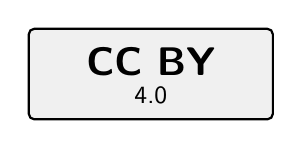
\begin{tikzpicture}
    \draw[rounded corners=2pt,line width=0.8pt,fill=black!6] (0,0) rectangle (3.1,1.15);
    \node[font=\bfseries\sffamily\Large] at (1.55,0.73) {CC BY};
    \node[font=\sffamily\small] at (1.55,0.30) {4.0};
  \end{tikzpicture}
\end{minipage}\hfill
\begin{minipage}[c]{0.64\textwidth}
  \small\sffamily
  AJbook 核心与封面标题框架源自 Wen-Wei Li（李文威）的 AlJabr-1，依
  CC BY 4.0 修改；永久 Tag 网络由本项目重绘。中文译文依 GNU Free
  Documentation License 1.2 或更高版本分发；详见正文来源页及仓库许可证文件。
\end{minipage}

\cleardoublepage
\end{titlepage}
